\documentclass[11pt]{article}
\usepackage[margin=1in]{geometry}
\usepackage{mathpazo}
\usepackage{amsmath,amssymb}
\usepackage{microtype}
\usepackage{booktabs}
\usepackage{graphicx}
\usepackage[dvipsnames]{xcolor}
\usepackage{tikz}
\usetikzlibrary{positioning,arrows.meta,calc,fit,backgrounds}
\usepackage[most]{tcolorbox}
\usepackage{enumitem}
\usepackage{listings}
\usepackage[font=small,labelfont=bf]{caption}
\usepackage{hyperref}
\hypersetup{colorlinks=true,linkcolor=MidnightBlue,citecolor=MidnightBlue,urlcolor=MidnightBlue}
\usepackage{cleveref}
\urlstyle{tt}
\def\UrlBreaks{\do\_\do/\do.}
\newcommand{\file}[1]{\nolinkurl{#1}}
\newcommand{\code}[1]{\texttt{#1}}
\newcommand{\mhh}{m_{hh}}
\newcommand{\bw}{\boldsymbol{\omega}}
\newcommand{\bp}{\boldsymbol{p}}
\newcommand{\bx}{\boldsymbol{x}}
\newcommand{\data}{\mathcal{D}}

\definecolor{trainable}{HTML}{1B6CA8}
\definecolor{physics}{HTML}{2E933C}
\definecolor{datac}{HTML}{7B4EA3}
\definecolor{warn}{HTML}{C0392B}

\newtcolorbox{keyidea}[1][]{enhanced,breakable,colback=physics!6,colframe=physics!70!black,
  fonttitle=\bfseries,title={#1},boxrule=0.6pt,arc=2pt,left=6pt,right=6pt}
\newtcolorbox{aside}[1][]{enhanced,breakable,colback=trainable!5,colframe=trainable!70!black,
  fonttitle=\bfseries,title={#1},boxrule=0.6pt,arc=2pt,left=6pt,right=6pt}
\newtcolorbox{assume}[1][]{enhanced,breakable,colback=datac!5,colframe=datac!70!black,
  fonttitle=\bfseries,title={#1},boxrule=0.6pt,arc=2pt,left=6pt,right=6pt}
\newtcolorbox{watch}[1][]{enhanced,breakable,colback=warn!5,colframe=warn!70!black,
  fonttitle=\bfseries,title={#1},boxrule=0.6pt,arc=2pt,left=6pt,right=6pt}
\setlist{itemsep=2pt,topsep=3pt}
\setlength{\emergencystretch}{3em}

\lstset{language=Python, basicstyle=\ttfamily\small, columns=fullflexible,
  keepspaces=true, commentstyle=\color{physics!70!black}\itshape,
  keywordstyle=\color{trainable!90!black}\bfseries, stringstyle=\color{datac},
  showstringspaces=false, frame=single, rulecolor=\color{gray!40},
  backgroundcolor=\color{gray!3}, xleftmargin=4pt, xrightmargin=4pt,
  aboveskip=6pt, belowskip=6pt}

\title{\textbf{A Bayesian neural network for \texttt{dihiggs}}\\[4pt]
\large Hamiltonian Monte Carlo after Radford Neal: the module \texttt{hmc.py}\\
\large and the notebook \texttt{heft\_train\_bnn.ipynb}\\[4pt]
\normalsize Plan, for approval before any code is written}
\date{October 29, 2026}

\begin{document}
\maketitle

\begin{abstract}
\noindent
This plan describes how to turn the \code{HEFTNet} model of the di-Higgs cross
section into a \emph{Bayesian neural network} (BNN) in the sense of Radford
Neal~\cite{neal1996,neal2011}. Instead of a single best set of parameters, a BNN is
an ensemble of parameter sets drawn from the posterior density of the parameters
given the training data. The draws are made with Hamiltonian Monte Carlo (HMC),
implemented from scratch in a new, model-agnostic Python module, \file{hmc.py}, which
uses PyTorch only to compute gradients. The module finds a model's parameters by
itself, groups them as Neal does, samples them, and writes each sampled parameter set
to its own \file{params_NNNN.pth} file in a run folder. A companion class, \code{BNN},
reads those files back and computes the posterior mean of the network output, its
standard deviation, quantiles and intervals. The module starts life in
\file{dihiggs/} and is written so that it can move to \code{drwho} unchanged. A new
notebook, \file{code/heft_train_bnn.ipynb}, in the style of \file{heft_train.ipynb},
drives it. Nothing will be written until you approve; the decisions needed are
collected in \cref{sec:decisions}.
\end{abstract}

\begin{keyidea}[The proposal in brief]
\begin{enumerate}
  \item \textbf{What is sampled.} The posterior density
    $p(\bw, \tau, b \mid \data)$ of the 3,944 network parameters $\bw$, the
    prior precisions $\tau$ of Neal's 16 parameter groups, and the noise scale $b$.
  \item \textbf{How.} HMC for $\bw$ (gradients from PyTorch autograd), alternated
    with exact Gibbs draws of $\tau$ and $b$, as in Neal's own software.
  \item \textbf{Likelihood.} By default a Laplace likelihood, the probabilistic
    counterpart of the L1 loss we already train with. Its most probable point is
    exactly our current training with weight decay added.
  \item \textbf{Start.} From the trained L1 model (a \emph{warm start}), so that the
    chain begins where the posterior mass is, instead of spending most of the
    computing time getting there.
  \item \textbf{Output.} \file{runs/BNN_<likelihood>/samples/params_0001.pth},
    \file{params_0002.pth}, \ldots, each an ordinary \code{state\_dict} that
    \code{HEFTNet().load()} reads, so the existing test and export notebooks
    work with any single sample.
  \item \textbf{Validation first.} The sampler is checked on a toy problem whose
    posterior is known exactly before it is let loose on \code{HEFTNet}.
\end{enumerate}
\end{keyidea}

\tableofcontents

% ===========================================================================
\section{What will be delivered}
\label{sec:deliver}

\begin{center}
\small
\begin{tabular}{p{0.34\textwidth}p{0.60\textwidth}}
\toprule
file & what it is\\
\midrule
\file{dihiggs/hmc.py} & the module: parameter discovery, priors, likelihoods,
  the posterior, the HMC sampler, the \code{BNN} ensemble and convergence
  diagnostics. Depends only on \code{torch}, \code{numpy} and the Python standard
  library (plus \code{pyyaml}, already a dependency).\\
\file{code/heft_train_bnn.ipynb} & the notebook that samples the \code{HEFTNet}
  posterior and plots the results, in the style of \file{heft_train.ipynb}\\
\file{code/hmc_toy.ipynb} & (if you agree, \cref{sec:decisions}) checks of the
  sampler on two small problems, one with an exactly known posterior\\
\file{docs/bnn/bnn_plan.pdf} & this document\\
\bottomrule
\end{tabular}
\end{center}

\noindent Every line of \file{hmc.py} will be commented for readers who know
Python and statistics but not PyTorch's internals: what each tensor holds, its
shape, and why each step is done. Constructs that tend to confuse (in-place
operations, \code{torch.no\_grad()}, \code{detach()}, slicing of flat vectors,
generators) will each get a short explanation where they are first used.

% ===========================================================================
\section{The Bayesian neural network}
\label{sec:bnn}

\subsection{From one best fit to an ensemble}

At present, training finds one parameter vector $\bw^*$ by minimising the empirical
risk, and the cross section is predicted as $f(\bx; \bw^*)$, with
$\bx = (\mhh, \kappa_\lambda, c_t, c_{tt}, c_{ggh}, c_{gghh})$. Neal's
idea~\cite{neal1996} is to treat $\bw$ like any other unknown parameter in a
Bayesian analysis. Bayes' theorem gives the posterior density
\begin{equation}
  p(\bw \mid \data) = \frac{p(\data \mid \bw)\, \pi(\bw)}{p(\data)},
  \qquad \data = \{(\bx_i, t_i),\ i = 1,\ldots,N\},
  \label{eq:bayes}
\end{equation}
where $p(\data \mid \bw)$ is the likelihood, $\pi(\bw)$ the prior and $t_i$ the
POWHEG cross section in a bin. The prediction at a new point $\bx$ is then not a
single number but the posterior mean, with its spread:
\begin{equation}
  \bar f(\bx) = \int f(\bx; \bw)\, p(\bw \mid \data)\, d\bw
  \;\approx\; \frac{1}{K} \sum_{k=1}^{K} f(\bx; \bw_k),
  \qquad \bw_k \sim p(\bw \mid \data).
  \label{eq:mean}
\end{equation}
The integral over 3,944 dimensions cannot be done directly. It is approximated by
an average over $K$ parameter vectors $\bw_1, \ldots, \bw_K$ \emph{sampled} from
the posterior. Those samples are what the HMC sampler produces, and what is stored
in the \file{params_NNNN.pth} files. In the same way, the standard deviation of
$f(\bx; \bw_k)$ over $k$ measures how well the data determine the function at
$\bx$, and its quantiles give credible intervals.

\begin{aside}[What the band means, and what it does not]
The spread of $f(\bx; \bw_k)$ is the \emph{epistemic} uncertainty: how much the
function could vary given the finite, noisy training data and the flexibility of
the network. We expect it to be small where the training data are dense and larger
where they are sparse or where the model struggles, e.g.\ just above threshold.
It is \emph{not} an uncertainty on POWHEG, nor on the HEFT calculation itself.
With about 274,000 training rows, the posterior will be narrow, and the band may
well be smaller than the POWHEG noise almost everywhere. Finding out where it is
not is one of the useful results of the exercise.
\end{aside}

\subsection{The prior, following Neal}
\label{sec:prior}

Neal groups the parameters of a network by role and gives each group $g$ its own
Gaussian prior, whose width is itself unknown~\cite[ch.~2 and 3]{neal1996}:
\begin{equation}
  \bw_g \mid \tau_g \sim \mathcal{N}\!\left(0,\ \tau_g^{-1} I\right), \qquad
  \tau_g \sim \text{Gamma}(\alpha_g, \beta_g).
  \label{eq:prior}
\end{equation}
Here $\tau_g$ is the \emph{precision} (one over the variance) of group $g$, and
$\alpha_g, \beta_g$ are the shape and rate of its Gamma prior. Such a
\emph{hierarchical} prior lets the data decide how large the weights of each layer
should be, instead of fixing that by hand. In \code{HEFTNet} there are 16 groups,
one per parameter tensor (\cref{tab:groups}); the module finds them automatically
(\cref{sec:view}).

\begin{table}[h]
\centering\small
\begin{tabular}{llrl}
\toprule
group (PyTorch name) & role & size & default prior scale $\sigma_g$\\
\midrule
\code{P.0.weight}, \code{P.0.bias} & input ($\mhh$) $\to$ hidden 1 & 25 + 25 & $1/\sqrt{1}$, 1\\
\code{P.2.weight}, \code{P.2.bias} & hidden 1 $\to$ hidden 2 & 625 + 25 & $1/\sqrt{25}$, 1\\
\quad$\vdots$ & \quad$\vdots$ (hidden layers 3 to 6) & & \\
\code{P.12.weight}, \code{P.12.bias} & hidden 6 $\to$ 23 outputs ($\tanh$) & 575 + 23 & $1/\sqrt{25}$, 1\\
\code{Q.weight}, \code{Q.bias} & $\mhh \to$ 23 exponents & 23 + 23 & 1, 1\\
\midrule
16 groups & & 3,944 & \\
\bottomrule
\end{tabular}
\caption{The parameter groups of \code{HEFTNet}. The indices 0, 2, \ldots, 12 are
the positions of the \code{nn.Linear} layers inside \code{nn.Sequential}; the odd
positions hold the activation functions, which have no parameters. The proposed
default prior mean of $\tau_g$ is $1/\sigma_g^2$, with $\sigma_g = 1/\sqrt{\text{fan-in}}$
for weights (Neal's scaling, which keeps the prior on the function sensible as the
width grows~\cite[ch.~2]{neal1996}) and $\sigma_g = 1$ for biases.}
\label{tab:groups}
\end{table}

\begin{aside}[Why the hyperparameters can be drawn exactly (Gibbs sampling)]
Given the current weights $\bw_g$ (with $n_g$ elements), the density of $\tau_g$ is
\[
p(\tau_g \mid \bw_g) \propto
\underbrace{\tau_g^{n_g/2} e^{-\tau_g \lVert\bw_g\rVert^2/2}}_{\text{Gaussian prior on }\bw_g}
\;\underbrace{\tau_g^{\alpha_g - 1} e^{-\beta_g \tau_g}}_{\text{Gamma prior}}
= \tau_g^{(\alpha_g + n_g/2) - 1}\, e^{-(\beta_g + \lVert\bw_g\rVert^2/2)\,\tau_g},
\]
which is again a Gamma density, with shape $\alpha_g + n_g/2$ and rate
$\beta_g + \lVert\bw_g\rVert^2/2$. (A prior with this property is called
\emph{conjugate}.) A new $\tau_g$ can therefore be drawn exactly with
\code{torch.distributions.Gamma}, with no tuning and no rejection. Neal's software
alternates such Gibbs draws of the hyperparameters with HMC updates of the
weights~\cite{neal1996}; we do the same.
\end{aside}

\subsection{The likelihood}
\label{sec:likelihood}

The likelihood says how the POWHEG value $t_i$ scatters about the network's
prediction $f_i = f(\bx_i; \bw)$. Three choices will be offered through a switch,
\code{LIKELIHOOD}:

\begin{center}
\small
\begin{tabular}{lllp{0.36\textwidth}}
\toprule
\code{LIKELIHOOD} & $-\log p(t_i \mid f_i)$ & counterpart & noise parameter\\
\midrule
\code{'laplace'} (default) & $\lvert t_i - f_i\rvert / b + \log 2b$ & L1 loss
  & one scale $b$ (pb), Gibbs-sampled (inverse-Gamma)\\
\code{'gaussian'} & $(t_i - f_i)^2 / 2s^2 + \log s$ & MSE loss
  & one variance $s^2$, Gibbs-sampled (inverse-Gamma)\\
\code{'poisson'} (experimental) & $(t_i - f_i)^2 / 2\sigma_i^2$ & CHI2 loss
  & none: $\sigma_i^2 = w_j t_i$ known from the event count\\
\bottomrule
\end{tabular}
\end{center}

\begin{keyidea}[The link with what we already do]
With the Laplace likelihood and the prior of \cref{eq:prior}, minus the log of the
posterior is
\[
  U(\bw) = \frac{1}{b} \sum_{i=1}^{N} \lvert t_i - f(\bx_i;\bw)\rvert
  \;+\; \sum_{g} \frac{\tau_g}{2}\, \lVert \bw_g \rVert^2 \;+\; \text{const}
  = \frac{N}{b}\left[ \underbrace{\frac{1}{N}\sum_i \lvert t_i - f_i\rvert}_{\text{our L1 empirical risk}}
  + \underbrace{\sum_g \frac{b\,\tau_g}{2N} \lVert\bw_g\rVert^2}_{\text{weight decay}} \right].
\]
So the most probable point of the posterior is the L1 training of
\file{heft_train.ipynb} with a (tiny, since $N$ is large) weight decay. The BNN
does not replace that training: it explores the neighbourhood of its answer, with
a width set by the data. That is why the trained L1 model is a natural starting
point for the sampler (\cref{sec:warm}).
\end{keyidea}

\begin{watch}[One noise scale for cross sections that span seven decades]
The Laplace and Gaussian likelihoods use a single noise scale $b$ (or $s$) for all
bins, just as L1 and MSE treat an error of $10^{-4}$~pb the same in every bin. The
fitted $b$ will be set by the large cross sections. The \emph{epistemic} band from
the spread of the $\bw_k$ is still meaningful, but a \emph{predictive} band that
adds noise of size $b$ will be too wide for small bins and too narrow for large
ones. The physically correct likelihood is \code{'poisson'}, with the known
variance $\sigma_i^2 = w_j t_i$ of a histogram of 40,000 events of weight $w_j$.
That is the CHI2 loss which trained poorly, probably because its weights span ten
decades. HMC will not cure that bad conditioning, so \code{'poisson'} is offered as
an experiment, not as the default.
\end{watch}

\noindent The Gibbs draw of the noise scale works exactly as for $\tau_g$. For the
Laplace likelihood with an inverse-Gamma prior $b \sim \text{InvGamma}(\alpha_b, \beta_b)$,
\[
  b \mid \bw, \data \sim \text{InvGamma}\Big(\alpha_b + N,\ \ \beta_b + \sum_i \lvert t_i - f_i\rvert\Big),
\]
and for the Gaussian, $s^2 \mid \bw, \data \sim \text{InvGamma}(\alpha_s + N/2,\ \beta_s + \sum_i (t_i - f_i)^2/2)$.

% ===========================================================================
\section{Hamiltonian Monte Carlo, step by step}
\label{sec:hmc}

\subsection{The idea}

Write the posterior as a Boltzmann distribution, $p(\bw \mid \data) \propto
e^{-U(\bw)}$, with the \emph{potential energy}
\begin{equation}
  U(\bw) = -\log p(\data \mid \bw) - \log \pi(\bw \mid \tau).
\end{equation}
HMC~\cite{duane1987,neal2011} pretends that $\bw$ is the position of a particle
moving on the surface $U$, and gives it a fictitious momentum $\bp$, one component
per parameter, with kinetic energy $K(\bp) = \tfrac12 \bp^{\mathsf T} M^{-1} \bp$,
where $M$ is a ``mass matrix'' (diagonal here). The joint density of $(\bw, \bp)$ is
$\propto e^{-H(\bw, \bp)}$ with $H = U + K$, so $\bw$ and $\bp$ are independent and
the marginal of $\bw$ is the posterior we want. Each HMC update has three steps:

\begin{enumerate}
  \item \textbf{Kick.} Draw a fresh momentum, $\bp \sim \mathcal{N}(0, M)$.
  \item \textbf{Glide.} Follow Hamilton's equations, $d\bw/ds = M^{-1}\bp$,
    $d\bp/ds = -\nabla U(\bw)$, for a fictitious time $L\varepsilon$, using $L$
    \emph{leapfrog} steps of size $\varepsilon$:
    \begin{align*}
      \bp &\leftarrow \bp - \tfrac{\varepsilon}{2}\, \nabla U(\bw) && \text{(half step in momentum)}\\
      \bw &\leftarrow \bw + \varepsilon\, M^{-1}\bp && \text{(full step in position)}\\
      \bp &\leftarrow \bp - \tfrac{\varepsilon}{2}\, \nabla U(\bw) && \text{(half step in momentum)}
    \end{align*}
    (consecutive half steps in momentum are merged, so each leapfrog step costs one
    gradient).
  \item \textbf{Accept or reject.} Exact dynamics would conserve $H$. Leapfrog does
    so only approximately, so the end point $(\bw', \bp')$ is accepted with
    probability $\min\{1, e^{-\Delta H}\}$, $\Delta H = H(\bw', \bp') - H(\bw, \bp)$.
    If it is rejected, the chain stays at $\bw$ (and $\bw$ is counted again).
\end{enumerate}

\noindent \Cref{fig:hmc} shows why this is worth the trouble. Neural-network
posteriors are full of long, narrow ridges. A random-walk sampler must take steps
no larger than the width of the ridge, so it diffuses along it slowly. An HMC
trajectory follows the ridge, because the gradient keeps pushing it back into the
valley, and in one update travels a distance comparable to the length of the ridge.
Along the way $U$ and $K$ exchange energy while $H$ stays nearly constant, so the
acceptance probability stays high.

\begin{figure}[h]
\centering
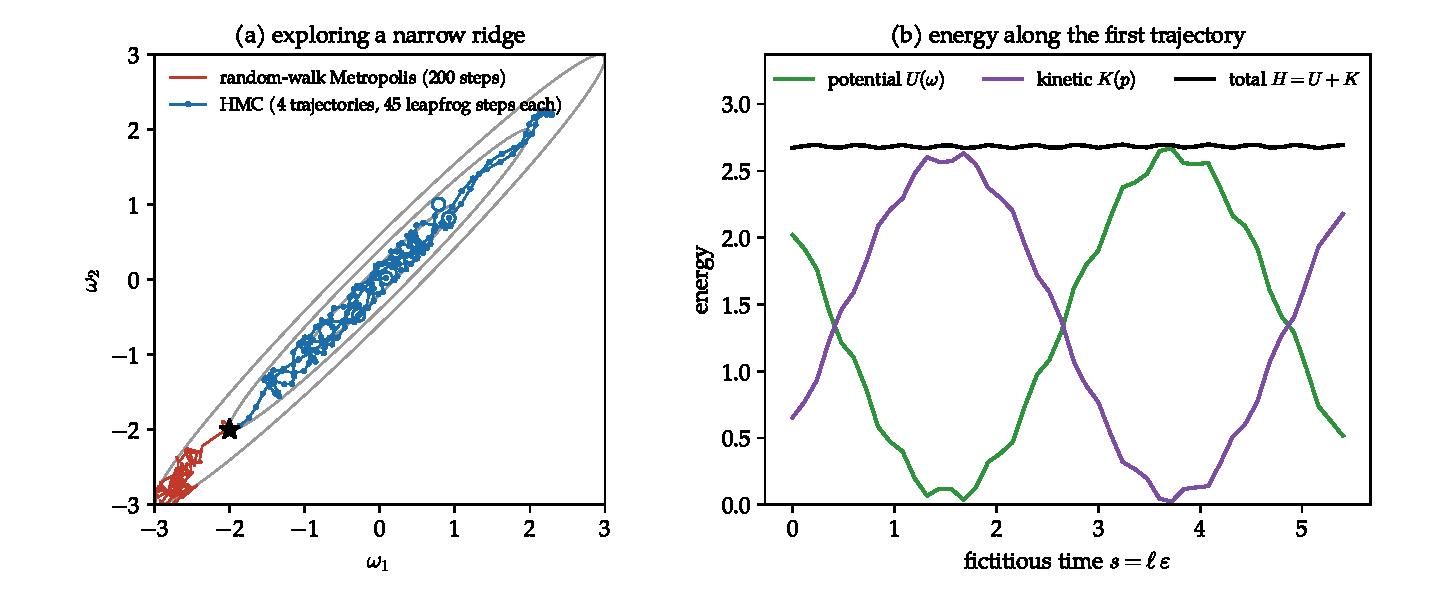
\includegraphics[width=\textwidth]{fig_hmc.pdf}
\caption{(a) Sampling a Gaussian with correlation 0.98, starting at the star.
200 random-walk Metropolis steps (red) barely move, while each of four HMC
trajectories (blue; open circles are the end points) crosses much of the ridge.
(b) Along one trajectory, potential and kinetic energy trade places while the total
energy $H$ is conserved to about 1\%, so the end point is almost always accepted.}
\label{fig:hmc}
\end{figure}

\begin{aside}[Why the result is exactly the posterior, and not an approximation]
The leapfrog map has two properties that hold whatever $\varepsilon$ is: it is
\emph{reversible} (run it again after flipping the sign of $\bp$ and you return to
the start) and it \emph{preserves volume} in $(\bw, \bp)$ space (each of the three
sub-steps is a shear, which changes one set of coordinates by an amount that depends
only on the other set). With these two properties, the accept/reject step makes the
chain satisfy detailed balance with respect to $e^{-H}$ exactly~\cite{neal2011}.
A large $\varepsilon$ only lowers the acceptance rate; it does not bias the samples.
Neither property needs $U$ to be smooth, so the kinks of $\lvert t - f\rvert$ and of
the ReLU are allowed; they merely make $\Delta H$ a little larger.
\end{aside}

\subsection{Tuning: step size, trajectory length, mass matrix}
\label{sec:tuning}

HMC has three settings. They are adjusted during a \emph{warm-up} phase, whose
samples are discarded, and then frozen, because changing them while sampling would
break the Markov property.

\begin{itemize}
  \item \textbf{Step size $\varepsilon$.} Too large: $\Delta H$ is large and most
    trajectories are rejected. Too small: each trajectory moves a short distance.
    During warm-up, $\varepsilon$ is adjusted by \emph{dual averaging}~\cite{hoffman2014}
    so that the average acceptance rate reaches a target (default 0.8): raised when
    the acceptance is above target, lowered when below, with an averaging that makes
    it settle. In the sampling phase each trajectory uses $\varepsilon$ times a random
    factor between 0.9 and 1.1 (``jitter''), as Neal recommends, to avoid trajectories
    that happen to return to their start.
  \item \textbf{Number of leapfrog steps $L$.} Fixed by the user (switch
    \code{N\_LEAPFROG}), also with a small random jitter. The diagnostics of
    \cref{sec:diagnostics} tell whether it is long enough.
  \item \textbf{Mass matrix $M$.} The leapfrog step in $\bw$ is $\varepsilon M^{-1}\bp$.
    If some parameters are far more tightly constrained than others, one $\varepsilon$
    cannot suit all of them. Setting $M^{-1}$ to the posterior \emph{variance} of each
    parameter, estimated from the second half of the warm-up, rescales every parameter
    to unit width~\cite{neal2011}. This is a diagonal matrix of 3,944 numbers.
\end{itemize}

\begin{assume}[What HMC requires of the problem]
\begin{enumerate}
  \item $U(\bw)$ and $\nabla U(\bw)$ can be computed (almost everywhere) for any $\bw$.
    PyTorch autograd supplies the gradient.
  \item The model is a \emph{deterministic} function of its inputs and parameters:
    no dropout and no batch normalisation. The module checks this.
  \item \textbf{Every gradient uses all $N$ training rows.} A gradient from a random
    mini-batch is noisy, and noisy gradients destroy the conservation of $H$ on which
    the accept/reject step relies. (Stochastic-gradient variants exist~\cite{chen2014},
    but they sample the posterior only approximately and are not Neal's method.)
    The sum over rows will be computed in chunks to bound memory; the sum of the
    chunks is exact.
\end{enumerate}
\end{assume}

% ===========================================================================
\section{Applying HMC to \texttt{HEFTNet}}
\label{sec:heftnet}

\subsection{Warm start}
\label{sec:warm}

Neal starts his chains from small random weights and lets them find the region of
high posterior density. With 274,000 rows, a full-data gradient per leapfrog step and
a narrow posterior, that ``burn-in'' would consume most of the computing time. The
proposal is therefore to start from the parameters of a trained L1 model (switch
\code{WARM\_START}, default \file{runs/L1Loss_ids/dihiggs_params.pth}), which is
close to the posterior mode (\cref{sec:likelihood}). The hyperparameters start at
values computed from those weights: $\tau_g = n_g/\lVert\bw_g\rVert^2$, and $b$
equal to the mean absolute residual. A short warm-up then lets the chain settle into
the posterior proper. Setting \code{WARM\_START = None} reproduces Neal's
start from the prior, for comparison.

\subsection{Cost}
\label{sec:cost}

Your full training run, 200,000 iterations of 2,048 rows in about 42 minutes on a
CPU, implies about 6\,$\mu$s per row for a forward and backward pass. A full-data
gradient therefore costs at most about 1.7~s on that CPU, and a trajectory of
$L = 100$ leapfrog steps about 3~minutes. 1,000 trajectories would take two days
on the CPU (an upper bound, since large batches use the CPU more efficiently than
batches of 2,048). On a GPU, where the 274,000 rows fit in one pass, a gradient
should take milliseconds, and the same run an hour or less. The notebook will
\emph{time} one gradient before sampling and print the predicted run time, so you
can choose \code{N\_LEAPFROG} and \code{N\_SAMPLES} knowingly. A switch
\code{DATA\_FRACTION} uses only a fraction of the training spectra (whole spectra,
not rows), for quick tests; the posterior is then wider, as it should be with less
data.

\begin{watch}[Things that can go wrong, and what the module does about them]
\begin{enumerate}
  \item \textbf{Bad conditioning.} Neural-network posteriors have directions that are
    constrained a million times more tightly than others. A diagonal mass matrix
    removes differences of scale between parameters but not correlations among them.
    If the acceptance is good but the samples are strongly autocorrelated, $L$ must
    grow. Large studies of full-data HMC for networks~\cite{izmailov2021} needed long
    trajectories; we should expect the same.
  \item \textbf{Precision.} $U$ is a sum of 274,000 terms of order 1 or more, while the
    accept/reject step needs $\Delta H$ to about 0.01. In single precision (about 7
    digits) the sum would be at the edge of that. The model will run in single
    precision, but $U$, $H$ and the chunk sums will be accumulated in double precision.
  \item \textbf{Divergences.} If $\Delta H$ exceeds 1,000, the trajectory has gone
    unstable (e.g.\ $e^{Q}$ in \code{HEFTNet} overflowed). It is rejected, counted,
    and reported; many divergences mean $\varepsilon$ is too large.
  \item \textbf{Symmetries.} Permuting the hidden units of a layer, or rescaling a
    ReLU unit's input weights by $c$ and its output weights by $1/c$, leaves $f$
    unchanged. Individual weights therefore need not converge, and are not
    monitored; only quantities that matter, $U$, the hyperparameters and predictions
    at chosen points, are.
\end{enumerate}
\end{watch}

% ===========================================================================
\section{The module \texttt{hmc.py}}
\label{sec:module}

\subsection{Design}

\Cref{fig:arch} shows the pieces and how data flow between them. Each piece is a
small class with one job. None of them knows anything about di-Higgs physics: the
model, the data and the likelihood are handed in. That is what will let the file move
to \code{drwho} unchanged.

\begin{figure}[h]
\centering
\resizebox{\textwidth}{!}{%
\begin{tikzpicture}[
  font=\small, >={Stealth[length=2.2mm]},
  box/.style={draw, rounded corners=2pt, thick, align=center, inner sep=3pt,
              minimum height=12mm, text width=30mm},
  usr/.style={box, fill=datac!8, draw=datac!80!black},
  mod/.style={box, fill=trainable!10, draw=trainable!80!black},
  res/.style={box, fill=physics!10, draw=physics!80!black, text width=36mm},
]
\node[usr] (model) at (0, 2.2)  {\code{HEFTNet()}\\\footnotesize any \code{nn.Module}};
\node[usr] (dat)   at (0, 0)    {training data\\\footnotesize tensors $X$, $t$};
\node[usr] (lik)   at (0, -2.2) {\code{LaplaceLikelihood}\\\footnotesize or Gaussian, Poisson};
\node[mod] (view)  at (4.2, 2.2) {\code{ParameterView}\\\footnotesize finds the 16 groups;\\\footnotesize model $\leftrightarrow$ flat $\bw$};
\node[mod] (prior) at (4.2, -2.2){\code{HierarchicalPrior}\\\footnotesize Neal's $\tau_g$; Gibbs};
\node[mod] (post)  at (8.4, 0)   {\code{Posterior}\\\footnotesize $U(\bw)$, $\nabla U(\bw)$\\\footnotesize (autograd, chunks)};
\node[mod] (hmc)   at (12.6, 0)  {\code{HMC}\\\footnotesize leapfrog, accept,\\\footnotesize warm-up, Gibbs};
\node[res] (run)   at (12.6, 2.6){\file{runs/BNN_laplace/}\\\footnotesize \file{samples/params_*.pth}\\\footnotesize trace, state};
\node[res] (bnn)   at (12.6, -2.6){\code{BNN}\\\footnotesize mean, std,\\\footnotesize quantiles, intervals};
\draw[->, thick] (model) -- (view);
\draw[->, thick] (view) -- (post);
\draw[->, thick] (dat) -- (post);
\draw[->, thick] (lik) -- (post);
\draw[->, thick] (prior) -- (post);
\draw[->, thick] (view) -- (prior);
\draw[->, thick] (post) -- (hmc);
\draw[->, thick] (hmc) -- node[right, font=\footnotesize]{writes} (run);
\draw[->, thick] (run.east) -- ++(0.6,0) |- node[pos=0.25, right, font=\footnotesize]{reads} (bnn.east);
\end{tikzpicture}}
\caption{The classes of \file{hmc.py} (blue), what the user provides (purple) and what
the sampler produces (green).}
\label{fig:arch}
\end{figure}

\subsection{Finding the parameters automatically}
\label{sec:view}

Every PyTorch model is an \code{nn.Module}, and every \code{nn.Module} can list its
own parameters, with their names, through \code{named\_parameters()}. That is all
\code{ParameterView} needs; it never looks inside the model's code. For
\code{HEFTNet} it finds the 16 tensors of \cref{tab:groups}, by name and shape,
and by default makes each tensor a group of Neal's prior. It also provides the two
conversions HMC needs: from the model's tensors to one flat vector $\bw$ of 3,944
numbers (the ``position'') and back. A sketch, with comments of the kind the
final code will have:

\begin{lstlisting}
class ParameterView:
    def __init__(self, model):
        self.model = model
        self.names, self.params = [], []
        # named_parameters() walks through every sub-module of the model and
        # yields (name, tensor) pairs, e.g. ('P.0.weight', tensor of shape
        # [25, 1]), ('P.0.bias', tensor of shape [25]), ..., ('Q.bias', [23]).
        for name, p in model.named_parameters():
            if p.requires_grad:          # skip parameters frozen by the user
                self.names.append(name)
                self.params.append(p)
        # numel() = number of elements of a tensor, e.g. 25*25 = 625.
        self.sizes = [p.numel() for p in self.params]
        # where each tensor sits inside the flat vector: a list of slices,
        # e.g. 'P.0.weight' -> slice(0, 25), 'P.0.bias' -> slice(25, 50), ...
        ends = np.cumsum(self.sizes)
        self.slices = [slice(e - n, e) for e, n in zip(ends, self.sizes)]

    def get(self):
        # Copy all parameters into ONE flat vector (the HMC "position").
        # detach() cuts the link to the autograd history; clone() makes an
        # independent copy, so changing it does not change the model.
        return parameters_to_vector(self.params).detach().clone()

    def set(self, w):
        # Write a flat vector back into the model's tensors, in place.
        vector_to_parameters(w, self.params)
\end{lstlisting}

\noindent The gradient $\nabla U$ is obtained the same way: compute $U$ with the
model's parameters set to $\bw$, call \code{U.backward()}, and collect each
parameter's \code{.grad} into a flat vector in the same order. Groups can also be
chosen coarser (\code{grouping='all'}: one $\tau$ for every parameter) or by an
explicit dictionary from names to groups.

\paragraph{What a model must satisfy.} It is a \code{torch.nn.Module}; its
\code{forward} takes a tensor of inputs and returns one prediction per row; it has no
dropout or batch-normalisation layers (\code{ParameterView} inspects
\code{model.modules()} and stops with an explanation if it finds one); and it can be
rebuilt by calling its class with no arguments, so that \code{BNN} can recreate it.
\code{HEFTNet} satisfies all four, as does \code{drwho}'s \code{FCNN}.

\subsection{The classes and their methods}

\begin{center}
\small
\begin{tabular}{p{0.24\textwidth}p{0.70\textwidth}}
\toprule
class & main methods\\
\midrule
\code{ParameterView} & \code{get()}, \code{set(w)}, \code{grad()}, \code{groups},
  \code{summary()} (prints the table of groups)\\
\code{HierarchicalPrior} & \code{neg\_log(w)} $= \sum_g \tau_g\lVert\bw_g\rVert^2/2$;
  \code{gibbs(w)}: new $\tau_g$; \code{from\_weights(w)}: initial $\tau_g$\\
\code{LaplaceLikelihood}, \code{GaussianLikelihood}, \code{PoissonLikelihood} &
  \code{neg\_log(f, t)}; \code{gibbs(residuals)}: new noise scale (not for Poisson);
  \code{sample(f)}: simulated data, for predictive bands\\
\code{Posterior} & \code{U(w)}, \code{U\_and\_grad(w)}: sum over chunks of rows, in
  double precision; \code{time\_gradient()}\\
\code{HMC} & \code{run(n\_warmup, n\_samples, thin)}; \code{resume()};
  \code{acceptance\_rate()}; internally \code{leapfrog()}, \code{trajectory()},
  \code{adapt\_step\_size()}, \code{adapt\_mass()}\\
\code{BNN} & \code{predict(x)} $\to$ tensor $[K, N]$; \code{mean(x)}, \code{std(x)},
  \code{quantiles(x, q)}, \code{interval(x, cl)}, \code{predictive(x)} (adds the
  likelihood noise), \code{apply(fn, x)} (any function of a model, e.g.\ the
  coefficient functions \code{model.coeffs}), \code{len(bnn)}\\
functions & \code{autocorrelation(y)}, \code{ess(y)} (effective sample size),
  \code{rhat(chains)} (Gelman--Rubin)\\
\bottomrule
\end{tabular}
\end{center}

\noindent For many points (e.g.\ all 274,000 training rows), \code{mean} and
\code{std} are accumulated one sample at a time (Welford's running formulae), so the
$K \times N$ table of predictions is never held in memory. A typical use:

\begin{lstlisting}
from dihiggs import hmc
from dihiggs import heftnet as NN

bnn = hmc.BNN(NN.HEFTNet, 'runs/BNN_laplace')  # reads every params_NNNN.pth
mu  = bnn.mean(x)                  # posterior mean of sigma, one per row of x
sd  = bnn.std(x)                   # its posterior standard deviation
lo, hi = bnn.interval(x, cl=0.68)  # central 68% credible interval
A   = bnn.apply(lambda m, x: m.coeffs(x[:, 0]), x)  # samples of a_i(m_hh)
\end{lstlisting}

\subsection{The run folder}
\label{sec:runfolder}

\begin{center}
\small
\begin{tabular}{p{0.38\textwidth}p{0.56\textwidth}}
\toprule
file & contents\\
\midrule
\file{runs/BNN_laplace/dihiggs_config.yaml} & every setting (\code{drwho} \code{Config}),
  the warm-start file and the training file's SHA-256, as in \file{heft_train}\\
\file{dihiggs_hmc_trace.csv} & one row per trajectory: iteration, phase (warm-up or
  sampling), accepted?, $\Delta H$, $U$, $\varepsilon$, $L$, $b$, $\tau_1 \ldots \tau_{16}$\\
\file{dihiggs_hmc_state.pth} & checkpoint, rewritten every few minutes: current $\bw$,
  $\tau$, $b$, $\varepsilon$, $M$, iteration, random-number-generator states\\
\file{samples/params_0001.pth}, \ldots & one sampled parameter set each, a plain
  \code{state\_dict}, readable by \code{HEFTNet().load(file)}\\
\file{samples/index.csv} & for each sample: file name, iteration, $U$, $b$, $\tau_g$\\
\bottomrule
\end{tabular}
\end{center}

\noindent A sample is about 16~kB, so 1,000 samples take 16~MB. Because of the
checkpoint, a run interrupted by Colab, a time limit on the RTX~5090 cluster, or a
closed laptop lid continues with \code{sampler.resume()} from where it stopped, and
the result is the same as an uninterrupted run with the same seed. With
\code{N\_CHAINS} $> 1$, each chain gets its own sub-folder, \file{chain_1/},
\file{chain_2/}, \ldots, and its own seed; \code{BNN} pools them.

% ===========================================================================
\section{The notebook \texttt{heft\_train\_bnn.ipynb}}
\label{sec:notebook}

The notebook follows \file{heft_train.ipynb} cell for cell where it can (header with
\code{Created}/\code{Updated} lines, Colab set-up cell with \code{USE\_DRIVE},
imports, device, data loading with the SHA-256 fingerprint), then:

\begin{enumerate}
  \item \textbf{Introduction} (markdown): the BNN, the posterior, HMC, and the link to
    the L1 training, condensed from \cref{sec:bnn,sec:hmc}.
  \item \textbf{Switches} (defaults shown): \code{LIKELIHOOD = 'laplace'};
    \code{WARM\_START}; \code{N\_WARMUP = 500}; \code{N\_SAMPLES = 1000};
    \code{THIN = 1}; \code{N\_LEAPFROG = 100}; \code{TARGET\_ACCEPT = 0.8};
    \code{N\_CHAINS = 1}; \code{DATA\_FRACTION = 1.0}; \code{SEED = 42}.
    The run folder is \code{DIRNAME} = \file{BNN_<likelihood>}.
  \item \textbf{Model and parameters}: build \code{HEFTNet}, load the warm start, and
    print \code{ParameterView.summary()}, i.e.\ \cref{tab:groups} as found by the code.
  \item \textbf{Posterior}: prior, likelihood, \code{Posterior}; time one gradient;
    print the predicted run time.
  \item \textbf{Sample}: \code{HMC(...).run(...)}, with a progress line per
    trajectory (acceptance so far, $\varepsilon$, $U$, $b$); \code{RESUME = True}
    continues an interrupted run.
  \item \textbf{Diagnostics} (\cref{sec:diagnostics}): traces, acceptance,
    autocorrelation, effective sample size, $\hat R$ if several chains.
  \item \textbf{Results}: the BNN mean against POWHEG on the quick test rows (the
    scatter plot of \file{heft_train}); a few test spectra with the posterior mean and
    68\% and 95\% bands; the 23 coefficient functions $a_i(\mhh)$ with their bands;
    and the BNN mean compared with the warm-start L1 model.
\end{enumerate}

% ===========================================================================
\section{Validation}
\label{sec:validation}

\subsection{The sampler on problems with known answers}

Before \code{HEFTNet}, \file{code/hmc_toy.ipynb} (seconds on a CPU) runs:
\begin{enumerate}
  \item \textbf{Bayesian linear regression}, a ``network'' with one linear layer, a
    Gaussian prior of fixed precision and Gaussian noise of known variance. The posterior
    is then Gaussian with a mean and covariance that can be written down. The sampled
    means and covariances must agree with them within their Monte Carlo errors
    (computed from the effective sample size). This tests the leapfrog integrator, the
    accept/reject step, the mass matrix and the bookkeeping of \code{ParameterView}.
  \item \textbf{Neal's one-dimensional example}~\cite{neal1996}: a small network fitted
    to noisy points of a smooth curve on part of an interval, with the hierarchical
    prior and Gibbs updates switched on. The posterior band should hug the data where
    there are data and widen outside. This is a visual check of the whole machinery,
    and a good teaching example.
\end{enumerate}

\subsection{Diagnostics for the \texttt{HEFTNet} run}
\label{sec:diagnostics}

\begin{itemize}
  \item \textbf{Acceptance rate} in the sampling phase between about 0.6 and 0.9, and
    no (or very few) divergences.
  \item \textbf{Stationarity}: the traces of $U$, $b$ and the $\tau_g$ show no drift
    after warm-up.
  \item \textbf{Mixing}: the autocorrelation of $U$, and of the prediction at a handful
    of monitor points (e.g.\ the first bin above threshold and a bin near 1~TeV for the
    Standard Model point), and from it the effective sample size; we aim for at least 100.
  \item \textbf{Several chains}, if run: Gelman--Rubin $\hat R < 1.05$ for the same
    quantities.
\end{itemize}

\subsection{What counts as success}

\begin{enumerate}
  \item The toy checks pass.
  \item The diagnostics above are met for \code{HEFTNet}.
  \item The BNN mean is at least as accurate on the holdout spectra as the warm-start
    L1 model (median $\chi^2/N$ in \file{heft_test}), as expected of an average over
    nearby good fits.
  \item The bands are informative: they are wider where the model is known to be weak
    (near threshold) than where it is good. A coverage check (how often POWHEG's
    holdout value falls inside the predictive interval) is reported, with the caveat of
    the watch box in \cref{sec:likelihood} for the single-scale likelihoods.
\end{enumerate}

% ===========================================================================
\section{Moving the module to \texttt{drwho}}
\label{sec:drwho}

\file{hmc.py} will import nothing from \code{dihiggs}. Moving it means copying it to
\file{drwho/drwho/hmc.py}, adding \code{"hmc"} to the list of lazily loaded
submodules in \file{drwho/__init__.py}, and bumping the version, following the release
protocol of \file{docs/drwho-scheme.pdf}. In \code{dihiggs}, \file{dihiggs/hmc.py} can
then shrink to one line, \code{from drwho.hmc import *}, so the notebooks keep working;
or the notebooks can import from \code{drwho} directly. The \code{drwho} commit is yours.

% ===========================================================================
\section{Not in this plan}
\begin{itemize}
  \item No change to \file{heft_train.ipynb}, \file{heft_test.ipynb},
    \file{heft_checks.ipynb}, \file{heft_export.ipynb}, \file{heftnet.py} or the data.
  \item A BNN version of \file{heft_test.ipynb} (band-aware $\chi^2$, coverage per
    $\mhh$ bin) and an export of the ensemble to numpy/C++ are natural next steps,
    to be planned after we see the first results.
  \item The No-U-Turn sampler~\cite{hoffman2014}, which chooses $L$ automatically, is
    not Neal's method and is left out; it could be added later.
  \item Stochastic-gradient samplers~\cite{chen2014} and ``cold posteriors''
    (raising the likelihood to a power~\cite{wenzel2020}) are left out: they do not
    sample the posterior of \cref{eq:bayes}.
  \item Nothing is committed to git.
\end{itemize}

% ===========================================================================
\section{Decisions for you}
\label{sec:decisions}

\begin{keyidea}[Decisions before I proceed]
\begin{enumerate}
  \item \textbf{Likelihood.} Laplace as the default, Gaussian and Poisson (experimental)
    as options. Agreed?
  \item \textbf{Prior.} Neal's hierarchical Gaussian, one $\tau_g$ per tensor (16 groups),
    Gamma hyperpriors of shape $\alpha_g = 1$ with prior mean $1/\sigma_g^2$ as in
    \cref{tab:groups}, Gibbs updates after every trajectory. Agreed, or would you prefer
    fixed prior widths for a first version?
  \item \textbf{Warm start} from \file{runs/L1Loss_ids/} (your \file{runs/L1Loss/} would
    also do; it is only read, never written). Agreed?
  \item \textbf{Chains.} One chain by default, with \code{N\_CHAINS} available; or
    should the default be 4 chains, for $\hat R$, on the GPU?
  \item \textbf{File names.} \file{runs/BNN_<likelihood>/samples/params_0001.pth},
    four digits. Acceptable?
  \item \textbf{Toy notebook} \file{code/hmc_toy.ipynb}: include it? (Recommended: it is
    the only check that the sampler is right, and it would serve your students.)
  \item \textbf{Location of this document}: \file{docs/bnn/bnn_plan.pdf}?
\end{enumerate}
\end{keyidea}

% ===========================================================================
\begin{thebibliography}{9}
\bibitem{neal1996} R.~M.~Neal, \emph{Bayesian Learning for Neural Networks}, Lecture
  Notes in Statistics 118, Springer (1996).
\bibitem{neal2011} R.~M.~Neal, ``MCMC using Hamiltonian dynamics'', in \emph{Handbook of
  Markov Chain Monte Carlo}, eds.\ S.~Brooks \emph{et al.}, Chapman \& Hall/CRC (2011),
  arXiv:1206.1901.
\bibitem{duane1987} S.~Duane, A.~D.~Kennedy, B.~J.~Pendleton and D.~Roweth, ``Hybrid Monte
  Carlo'', Phys.\ Lett.\ B \textbf{195} (1987) 216.
\bibitem{hoffman2014} M.~D.~Hoffman and A.~Gelman, ``The No-U-Turn sampler: adaptively
  setting path lengths in Hamiltonian Monte Carlo'', J.\ Mach.\ Learn.\ Res.\ \textbf{15}
  (2014) 1593.
\bibitem{izmailov2021} P.~Izmailov, S.~Vikram, M.~D.~Hoffman and A.~G.~Wilson, ``What are
  Bayesian neural network posteriors really like?'', ICML 2021, arXiv:2104.14421.
\bibitem{chen2014} T.~Chen, E.~B.~Fox and C.~Guestrin, ``Stochastic gradient Hamiltonian
  Monte Carlo'', ICML 2014, arXiv:1402.4102.
\bibitem{wenzel2020} F.~Wenzel \emph{et al.}, ``How good is the Bayes posterior in deep
  neural networks really?'', ICML 2020, arXiv:2002.02405.
\end{thebibliography}

\end{document}
